\chapter{Antecedentes}
A partir de los estudios realizados por el Grupo de Investigación en Telemedicina de la Universidad Distrital Francisco José de Caldas se han detectado ciertas necesidades y obstáculos para el despliegue de redes de telemedicina. Con base en esto el \textbf{GITEM}, que ha sido pionero en el estudio y desarrollo de soluciones costo efectivas en el área de la telesalud, la teleducación y la administración de los servicios de salud, propone un sistema de información que integra, no solo los aspectos relacionados con la Telemedicina, sino también aquellos que tienen estrecha relación con las tecnologías necesarias para la implementación de los servicios y otros aspectos relevantes.

El proyecto recoge las experiencias que el grupo ha acumulado a través de más de siete años de trabajo continuo en el  área de la telemedicina y las aplica a modelos de gestión de conocimiento para formular una arquitectura conceptual y de software que contribuya a potenciar los ciclos de integración, creación, reproducción y diseminación del conocimiento; a través de un portal especializado.

El \textbf{Sistema de Información para Proyectos de Telemedicina}, conocido desde su primera versión con el nombre genérico de \textbf{SITEM}, es una herramienta de \textit{software libre} orientada a la web, que contiene subsistemas especializados para la gestión de información de diferentes componentes de las redes de telemedicina así como la definición de un modelo que provee los lineamientos para el desarrollo de módulos inéditos. En su más reciente versión explora la integración de \textit{Agentes} notificadores y de Recomendación que analizan constantemente los repositorios de información del sistema para, a partir de un proceso de minería de datos, desplegar información referenciada y adaptada a las necesidades y perfiles de cada uno de los usuarios registrados dentro del sistema. 

Propone un mecanismo para la integración de actores en el área del despliegue de soluciones de Telemedicina proveiendo un escenario ubicuo, basado en tecnologías de la información y un modelo de trabajo colaborativo en red que propende por la construcción evolutiva de una base de información y conocimiento que, asociados a los conceptos de libertad en el uso de la información y el conocimiento, busca elaborar un \textit{recurso público} esencial para el desarrollo de la Telemedicina y la Telesalud en la sociedad.

El modelo conceptual del SITEM aborda a la Telemedicina con un enfoque holístico que trasciende la mera dimensión técnica y tecnológica para abarcar también los aspectos médicos, culturales y de gestión de servicios de salud. Integra, en un solo ambiente, las herramientas básicas de gestión, focalización y orientación de información y conocimiento de diferentes componentes de las redes de Telemedicina que en el estado actual propone reglas formales de estructuración de los almacenes de datos y las bases de conocimiento. La arquitectura del SITEM incluye componentes esenciales para apoyar a los grupos de diseñadores y consultores en la ejecución de sus propuestas en el área que por la complejidad inherente no encuentran un producto que involucre de una forma unificada los diferentes aspectos que requieren ser considerados.

Es común que el desarrollo de soluciones basadas en software Telemédico deban pasar por un proceso de consultoría complejo, y costoso, que muchas entidades de salud son incapaces de costear; de igual manera la concentración de conocimiento en desarrollo de software, el descrédito infundado de soluciones alternativas deliberadamente generalizadas y el desconocimiento por parte de la alta gerencia de nuevas opciones de provisión de productos y servicios hace que todos los proyectos asociados a la Telemedicina y la telesalud parezcan como imposibles de alcanzar sin la inversión de exorbitantes sumas de dinero.
 
\section{Antecedentes del Dominio}
El estudio preliminar de diagnóstico desarrollado por el grupo de investigación GITEM a principios del milenio tenía en mente problemas puntuales para la implementación de servicios médicos prestados a través de medios teleinformáticos en el Distrito Capital\cite{aparicio2000}:

\begin{quote}
“En el momento no existe un diagnóstico real sobre los servicios requeridos en el área de telemedicina, razón suficiente para iniciar un trabajo de campo que establezca la situación actual de servicios médicos y la demanda real, así como la posibilidad de conocer a corto, mediano y largo plazo cuáles serían los costos de inversión que permitirían dar soluciones al problema  de cobertura.

La socialización del conocimiento alrededor de las tecnologías aplicadas al desarrollo de la medicina, es uno de los valores que lleva al éxito de soluciones efectivas en el sector salud, por tal motivo es necesario desarrollar un plan de alfabetización en el sector salud y en el sector gubernamental y académico.

En el país no existen estrategias de investigación en esta área del conocimiento para llevar a cabo un estudio real que permita dar el paso a soluciones verdaderas sobre desarrollo tecnológico o experimental para poder implementar centros de investigación en Telemedicina.

La Universidad Distrital tiene el recurso humano, el conocimiento y la experiencia científica y tecnológica, capaz de dar soluciones tangibles a estas necesidades; unida al conocimiento y experiencia de entidades como clínicas y hospitales  y con la participación de operadores de comunicaciones, puede desarrollar soluciones efectivas a los problemas de salud que afronta la sociedad colombiana.”
\end{quote}

Siendo el estudio totalmente eficaz dio surgimiento al despliegue de nuevos proyectos que aprovecharan de la mejor forma los resultados obtenidos que fueron recopilados en extensos tomos escritos y digitalizados. Para brindar una estructura formal a la documentación, brindar un acceso eficiente de entidades al estudio y gestionar los riesgos asociados al crecimiento de la complejidad a la hora de generar estudios comparativos o de apoyo a la toma de decisiones, se creó al interior del grupo un proyecto de grado denominado \textbf{Sistema de Información en Telemedicina} que en sus primeras fases de desarrollo dio solución parcial al marcar las pautas hacia la integración de información para el \textbf{GITEM} dejando además una investigación valiosa en el tema del desarrollo de software distribuido, interoperable y robusto basado en la filosofía del software libre.

De forma paralela el grupo de investigación implementó, en convenio con \textit{Colciencias}, el Sistema de Referencia y Contrarreferencia para el Distrito Capital, utilizando herramientas de desarrollo propietarias específicamente el middleware .NET de Microsoft con lo que el grupo adquirió experiencia en la desarrollo de aplicaciones siguiendo metodologías efectivas para la construcción de software.

Junto con estos proyectos se desarrolla actualmente cátedra en el área de la Telemedicina ofrecida como seminario inscrito dentro del plan de estudios de la \textit{Maestría en Ciencias de la Información y las Comunicaciones}, lo que ha fomentado el interés investigativo y la formación de profesionales especializados que ha contribuido a la construcción de nuevos saberes en la materia y que se demuestra en la cantidad creciente de proyectos asociados a la línea de investigación.

En la actualidad el grupo de investigación en telemedicina de la Universidad Distrital - \textbf{GITEM}, es catalogado por Colciencias como grupo clase A – el de más alto nivel, y el proyecto SITEM se encuentra institucionalizado por parte del Centro de Investigaciones y Desarrollo Científico con lo que se obtiene una posición de liderazgo en el tema de investigación y se reconoce el trabajo investigativo realizado por el grupo. Todos estos elementos ha generado una base de conocimiento tácito que evidentemente repercute en los sistemas desarrollados, promoviendo y presionando su crecimiento, la adaptación a nuevos requerimientos y el seguimiento de nuevos estándares y legislaciones.

\section{Fases Transcurridas en el SITEM}
En un primer acercamiento el proyecto de investigación se puede asociar a un holotipo proyectivo\cite{hurtado2000} cuyo estadio actual se ha logrado a partir de actividades investigativas que abordan distintos aspectos de la proyección, en la dimensión tecnológica, de los sistemas de Telemedicina. La idea fundamental que siempre ha guiado el proyecto es la de generar un proceso iterativo basado en la construcción y deconstrucción gradual, hermenéutico e incremental de un sistema informático que apoye las labores de consultoría y diseño de redes Telemédicas ahondando de forma asíncrona en cada uno de sus diferentes componentes. 

El proyecto tiene como particularidad tener que cumplir con ambiciosas metas de desarrollo con reducidos recursos técnicos y financieros los cuales deben ser administrados dentro de un ambiente de alta regulación burocrática. El escenario común ha sido el bajo tiempo de permanencia de los integrantes, la ejecución constante de tareas de capacitación, el uso intensivo de tecnologías de la comunicación, el teletrabajo  y la escasa interacción persona a persona. El \textbf{SITEM} inicialmente tenía que ser de calidad, económico y desarrollado rápidamente. Pero teniendo en cuenta lo que \cite{larman2003} nos citaba: “Rápido, barato, bueno: elija dos cualquiera”; con los pies firmemente puestos en el suelo,  dejando a un lado las fuertes esperanzas, debíamos sacrificar un aspecto y el único que se disponía era la rapidez en que versiones estables del proyecto habrían de ver la luz - los conceptos fundamentales de desarrollo de aplicaciones de software libre aportarían varias claves para minimizar el impacto de este sacrificio.

\begin{figure}
 \centering
 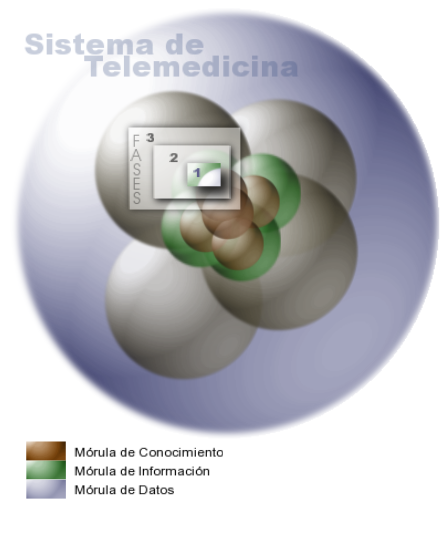
\includegraphics[width=156mm, height=195mm]{modelo_fases.png}
 \caption{Aproximación incremental a un sistema de Gestión de Conocimiento}
 \label{modelo1}
\end{figure}

Con esto como patrón fundamental el grupo de desarrollo plantea un modelo general en donde los objetivos de producir datos, consumir información y compartir conocimiento en el área de interés será alcanzado en varias fases\footnote{A través del presente documento se utilizan los términos de fase en el proceso investigativo y fases del Proceso de Desarrollo del Sistema Software. Las dos se suponen diferentes y su interpretación e importancia están asociados al contexto en el que se ubican.} de las cuales se describen los alcances de aquellas que han culminado.

La figura \ref{modelo1} muestra el proceso de estructuración de un sistema de telemedicina como una sucesión de fases que generan las dimensiones de datos, información y conocimiento de un grupo de componentes dado. El sistema visto como un \textit{holos} presenta al investigador una gran cantidad de datos que en la medida que se descubren, recolectan, observan y registran se van convirtiendo en información susceptible de ser descrita, analizada, integrada y comparada acercándose cada vez más a un conocimiento refinado. El carácter de discernible - el momento en que las dimensiones se solapan en grado sumo, se evidencia con el aumento colectivo de especialización en la materia y en nuestro caso, con el grado de inmersión de los usuarios en el SITEM.

En el transcurso de las fases solo se manejan ciertos aspectos que incremental y constructivamente se suman para crear un modelo cada vez más exacto del sistema con base en las diferentes \textit{mórulas} de datos, información y conocimiento generadas. Aunque en el gráfico se muestra un tanto discretos y exactos, los límites existentes entre las tres mórulas principales - datos, información, conocimiento; son en la realidad difusos. Esto dificulta la consecución del objetivo de cada fase que es tratar de profundizar en uno o varios componentes del holos - conseguir especificidad en el modelo.

Si se consideran los aspectos meramente técnicos del SITEM se corre el riesgo inminente de diseminación en regiones poco profundas del sistema - dispersión en la mórula de datos - razón por la cual la herramienta software se ha convertido en un artefacto intermedio y no en el fin último de la investigación.

\subsection{Sistema de Información para Telemedicina – Fase I}
Con la primera fase de desarrollo del SITEM se logró un conocimiento amplio de los componentes de las redes de telemedicina y sus interrelaciones basado en una investigación exploratoria y descriptiva realizada por los integrantes del grupo GITEM. 

También se determinaron las características esenciales de diferentes portales que implementaban en cierto grado la funcionalidad esperada para el SITEM vislumbrando con este estudio la necesidad de crear un producto software adaptado a las necesidades del entorno distrital, teniendo en cuenta que ninguno de los portales analizados brindaba acceso a información pertinente, confiable, actualizada y estructurada en torno a las redes de telemedicina en idioma español.

La cuestión fundamental que se resolvió en esta fase fue la definición de un modelo para la estructuración y administración de información relevante para los participantes en el diseño, análisis y desarrollo de las redes de Telemedicina. Además se definió un modelo de negocios que lograba mostrar las interrelaciones que tendría el sistema con los proyectos del grupo y un conjunto representativo de portales relacionados temáticamente; encontrando un costo de oportunidad adecuado. En la actualidad dicho modelo de negocios cobra mayor vigencia con la tendencia generalizada de desmonte de inversión en los portales más importantes a nivel mundial – siendo quizás \textbf{ipath}, también basado en la filosofía del software libre, uno de los únicos que continúan activos y en crecimiento, demostrando de paso que el esquema propuesto - gestionado eficientemente, es adecuado para el desarrollo y mantenimiento de sistemas de esta clase.

Al momento de desarrolló de esta fase el grupo de investigación no contaba ni siquiera con un portal web por lo que la arquitectura propuesta incluyó al portal del grupo como un subsistema del SITEM compartiendo de esta forma tanto la plataforma tecnológica como el modelo conceptual, lo que difuminó un poco los alcances reales del Sistema y su implementación no pasó de ser un prototipo de baja funcionalidad. 

Los alcances y logros efectivos de esta fase fueron:

\begin{itemize}
\item Descripción del Modelo de Negocio.
\item Propuesta de Desarrollo
\item Creación de la Arquitectura general del Sistema.
\item Desarrollo del sitio web del grupo GITEM e integración conceptual del SITEM dentro de los proyectos del grupo.
\item Elaboración de los Modelos básicos de Requisitos, análisis y diseño.
\item Estudios sobre filosofía de Software Libre.
\item Construcción de un Prototipo de baja funcionalidad conocido como SITEM versión 0.1, bautizada internamente como \textbf{Kauil}.
\end{itemize}


\begin{figure}
 \centering
 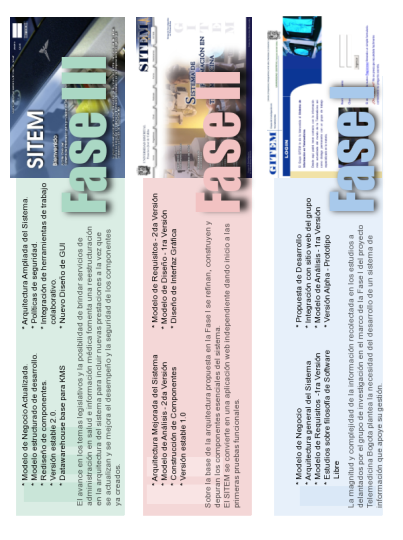
\includegraphics[width=142mm, height=190mm]{fase_sitem.png}
 \caption{Fases transcurridas en el desarrollo del SITEM}
 \label{fase_sitem}
\end{figure}

\subsection{Sistema de Información para Telemedicina – Fase II}

Los modelos de requisitos, análisis y diseño de la primera fase sirven de base para proponer arquitectura general para el Sistema de Información para Proyectos de Telemedicina y con el inicio de la segunda fase se emprenden las actividades necesarias para la construcción de los componentes de software que concretaban dicha arquitectura. Para poder minimizar los riesgos asociados al proyecto se adaptó el \textit{Proceso Unificado de Desarrollo de Software} a las especificidades de desarrollo del Sistema, lo que favoreció efectivamente su elaboración, implementación, mantenimiento y crecimiento.

La arquitectura general se vio poco afectada pero cada uno de los subsistemas componentes fueron más finadamente caracterizados resultando en un modelo de análisis y diseño mejor definido que integraba elementos no tratados en la fase inicial. Debido a la naturaleza del SITEM, el grupo de investigación decide separar los hilos de desarrollo del Sistema y del proceso de estructuración del sitio web del grupo. El SITEM por primera vez se puede acceder desde \textit{Internet} gracias al despliegue que se realiza sobre la plataforma de hardware y software brindada por la \textit{Universidad Distrital}. 

En esta fase se realiza el modelado de datos y se esbozan las primeras rutinas de manejo se seguridad. Para la construcción de componentes se utilizan herramientas de software libre y el grupo de desarrollo aumenta a cinco integrantes. El trabajo se encuentra, con excepción del director del proyecto, soportado y ejecutado por estudiantes de pregrado del proyecto curricular de Ingeniería Electrónica convirtiéndose en el \textbf{primer proyecto de desarrollo de software libre realizado por el GITEM} e involucra la formación transdisciplinar de un grupo de sus integrantes.

Los alcances de esta fase fueron:
\begin{itemize}
\item Arquitectura Mejorada del Sistema
\item Modelo depurado de Requisitos
\item Modelo de Análisis - Segunda Versión
\item Modelo de Diseño
\item Construcción de Componentes software soportado en su totalidad por herramientas de software libre.
\item Diseño de Interfaz Gráfica
\item Versión estable 1.0 y bautizada internamente como \textbf{Gucumatz}.
\item Adaptación del Proceso Unificado de Desarrollo de Software a las especificidades del SITEM.
\item Configuración de la plataforma tecnológica de despliegue del sistema.                                            \end{itemize}

Al final de la fase se obtiene un aplicativo que presenta avances en todos los subsistemas propuestos.


\subsection{Sistema de Información para Telemedicina – Fase III}

El almacén de datos obtenido en la segunda fase aunque interesante es poco funcional cuando se trata de aplicar directamente al apoyo de la implementación de soluciones basadas en software telemédico. Estos proyectos presentan retos adicionales en la medida que deben pasar por procesos de consultoría complejos y costosos que muchas entidades de salud públicas son incapaces de costear. Otros riesgos están asociados a la desinformación que injustificada y deliberadamente mantiene la empresa privada en cuanto a que con software libre no se siguen buenas prácticas de desarrollo de software, ni se obtienen sistemas seguros que garanticen la integridad de los datos - conceptos totalmente alejados de la realidad que pueden minar el juicio objetivo de administradores médicos no especializados en telemedicina - y mucho menos en teleinformática, en cuanto a la posibilidad de alcanzar sistemas eficientes y eficaces sin la inversión de exorbitantes sumas de dinero. 

Es común encontrar en el ámbito colombiano casos de éxito de aplicaciones telemédicas en entidades de salud privadas pero son escasas las aplicaciones en entidades públicas de segundo o tercer nivel. Evidentemente el uso, promoción y difusión de software libre es una práctica necesaria para poder implementar aplicaciones con altos niveles de calidad que beneficien al grueso de la población.

SITEM en esta fase genera una herramienta que ordena la información lógicamente y permite su acceso personalizado en áreas del conocimiento que tienen inferencia sobre las redes de telemedicina: medicina básica, tecnologías de interconexión, equipos de telemedicina, instituciones de salud, entidades prestadores de servicios de telecomunicaciones, entre otras; así mismo integra una serie de servicios en línea que propenden por la consolidación de una comunidad en Telemedicina basada en Internet, figura \ref{sitem_faseIII} .

Se consolida un proceso de desarrollo de software adaptado a las especificidades del grupo de investigación el cual trata de extraer lineamientos de las prácticas mundialmente aceptadas de procesos y métodos como son el Proceso Unificado, Métrica 5, Normas de Calidad ISO 9000 y EFQM. Se trata de buscar el aseguramiento de la calidad en el desarrollo, la interoperabilidad, escalabilidad y el uso extensivo de software libre. Se documenta todas las etapas involucradas en la creación de la aplicación para que sirva de plantilla a sistemas relacionados y se formaliza las áreas de capacitación a partir de ciclos genéricos de transferencia de conocimiento apoyados en tecnologías de la información.

\begin{figure}
 \centering
 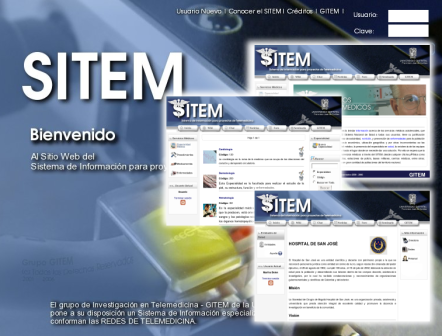
\includegraphics[width=156mm, height=118mm]{pagina_principal.png}
 \caption{Sistema de Información para proyectos de Telemedicina. Interfaz de Usuario en la Fase III}
 \label{sitem_faseIII}
\end{figure}